\documentclass[
  bibliography=totoc,     % Literatur im Inhaltsverzeichnis
  captions=tableheading,  % Tabellenüberschriften
  titlepage=firstiscover, % Titelseite ist Deckblatt
]{scrartcl}

% Paket float verbessern
\usepackage{scrhack}

% Warnung, falls nochmal kompiliert werden muss
\usepackage[aux]{rerunfilecheck}

% unverzichtbare Mathe-Befehle
\usepackage{amsmath}
% viele Mathe-Symbole
\usepackage{amssymb}
% Erweiterungen für amsmath
\usepackage{mathtools}

% Fonteinstellungen
\usepackage{fontspec}
% Latin Modern Fonts werden automatisch geladen
% Alternativ zum Beispiel:
%\setromanfont{Libertinus Serif}
%\setsansfont{Libertinus Sans}
%\setmonofont{Libertinus Mono}

% Wenn man andere Schriftarten gesetzt hat,
% sollte man das Seiten-Layout neu berechnen lassen
\recalctypearea{}

% deutsche Spracheinstellungen
\usepackage[ngerman]{babel}


\usepackage[
  math-style=ISO,    % ┐
  bold-style=ISO,    % │
  sans-style=italic, % │ ISO-Standard folgen
  nabla=upright,     % │
  partial=upright,   % │
  mathrm=sym,        % ┘
  warnings-off={           % ┐
    mathtools-colon,       % │ unnötige Warnungen ausschalten
    mathtools-overbracket, % │
  },                       % ┘
]{unicode-math}

% traditionelle Fonts für Mathematik
\setmathfont{Latin Modern Math}
% Alternativ zum Beispiel:
%\setmathfont{Libertinus Math}

\setmathfont{XITS Math}[range={scr, bfscr}]
\setmathfont{XITS Math}[range={cal, bfcal}, StylisticSet=1]

% Zahlen und Einheiten
\usepackage[
  locale=DE,                   % deutsche Einstellungen
  separate-uncertainty=true,   % immer Unsicherheit mit \pm
  per-mode=symbol-or-fraction, % / in inline math, fraction in display math
]{siunitx}

% chemische Formeln
\usepackage[
  version=4,
  math-greek=default, % ┐ mit unicode-math zusammenarbeiten
  text-greek=default, % ┘
]{mhchem}

% richtige Anführungszeichen
\usepackage[autostyle]{csquotes}

% schöne Brüche im Text
\usepackage{xfrac}

% Standardplatzierung für Floats einstellen
\usepackage{float}
\floatplacement{figure}{htbp}
\floatplacement{table}{htbp}

% Floats innerhalb einer Section halten
\usepackage[
  section, % Floats innerhalb der Section halten
  below,   % unterhalb der Section aber auf der selben Seite ist ok
]{placeins}

% Seite drehen für breite Tabellen: landscape Umgebung
\usepackage{pdflscape}

% Captions schöner machen.
\usepackage[
  labelfont=bf,        % Tabelle x: Abbildung y: ist jetzt fett
  font=small,          % Schrift etwas kleiner als Dokument
  width=0.9\textwidth, % maximale Breite einer Caption schmaler
]{caption}
% subfigure, subtable, subref
\usepackage{subcaption}

% Grafiken können eingebunden werden
\usepackage{graphicx}

% schöne Tabellen
\usepackage{tabularray}
\UseTblrLibrary{booktabs, siunitx}

% Verbesserungen am Schriftbild
\usepackage{microtype}

% Literaturverzeichnis
\usepackage[
  backend=biber,
]{biblatex}
% Quellendatenbank
\addbibresource{lit.bib}
\addbibresource{programme.bib}

% Hyperlinks im Dokument
\usepackage[
  german,
  unicode,        % Unicode in PDF-Attributen erlauben
  pdfusetitle,    % Titel, Autoren und Datum als PDF-Attribute
  pdfcreator={},  % ┐ PDF-Attribute säubern
  pdfproducer={}, % ┘
]{hyperref}
% erweiterte Bookmarks im PDF
\usepackage{bookmark}

% Trennung von Wörtern mit Strichen
\usepackage[shortcuts]{extdash}

\author{%
  Vincent Wirsdörfer\\%
  \href{mailto:vincent.wirsdoerfer@udo.edu}{authorA@udo.edu}%
  \and%
  Joris Daus\\%
  \href{mailto:joris.daus@udo.edu}{authorB@udo.edu}%
}
\publishers{TU Dortmund – Fakultät Physik}


\begin{document}
\section{Auswertung}
\label{sec:Auswertung}

In diesem Versuch wird das Geiger-Müller-Zählrohr vermessen. So werden typische Charakteristika wie die Kennlinie und 
die Totzeit bestimmt.

\subsection{Kennlinie des Geiger-Müller-Zählrohrs}
Um die Kennlinie zu vermessen, werden die Betriebsspannung und die Zählrate vermessen, wie in der Durchführung 
beschrieben. So werden die folgenden Werte aufgenommen:

\begin{table}[H]
    \caption{Messwerte der Spannung und der Zählrate auf 120s.}
    \label{tab:Kennlinie}
    \begin{minipage}[t]{0.5\textwidth}
        \vspace{0pt}
        \centering
    \begin{tblr}{
    colspec = {S[table-format=3.0] S[table-format=5.0]},
    row{1} = {guard, mode = math} 
    }
    \toprule
    \text{Spannung} \mathbin{/} \unit{\volt} & \text{Zählrate N} \\
    \midrule
        300 &   0       \\
        320 &   0       \\
        340 &   15380   \\
        360 &   15886   \\
        380 &   16143   \\
        400 &   16272   \\
        420 &   16317   \\
        440 &   16477   \\
        460 &   16430   \\
        480 &   16539   \\
        500 &   16429   \\
    \end{tblr}
\end{minipage}\hfill
\begin{minipage}[t]{0.5\textwidth}
    \vspace{0pt}
    \centering
    \begin{tblr}{
        colspec = {S[table-format=3.0] S[table-format=5.0]},
        row{1} = {guard, mode = math} 
        }
        \toprule
        \text{Spannung} \mathbin{/} \unit{\volt} & \text{Zählrate N} \\
        \midrule
            520 &   16620   \\
            540 &   16846   \\
            560 &   16814   \\
            580 &   16662   \\
            600 &   16736   \\
            620 &   16947   \\
            640 &   16680   \\
            660 &   16762   \\
            680 &   17101   \\
            700 &   17400   \\
            720 &   17790   \\
            740 &   18738   \\
        \end{tblr}
    \end{minipage}\hfill
\end{table}

\noindent Diese Daten können nun gegeneinander aufgetragen werden. Durch dann sichtbare Kennlinie 
des Zählrohrs kann das Arbeitsplateau bestimmt werden. 
Aus technischen Gründen misst das Zählrohr erst Teilchen ab einer Betriebsspannung von \qty{340}{\volt} 
Aus diesem Grund werden die ersten beiden Werte nicht mit in den Plot genommen.
So ergibt die folgende Kennlinie des Geiger-Müller-Zählrohrs.

\begin{figure}[H]
    \centering
    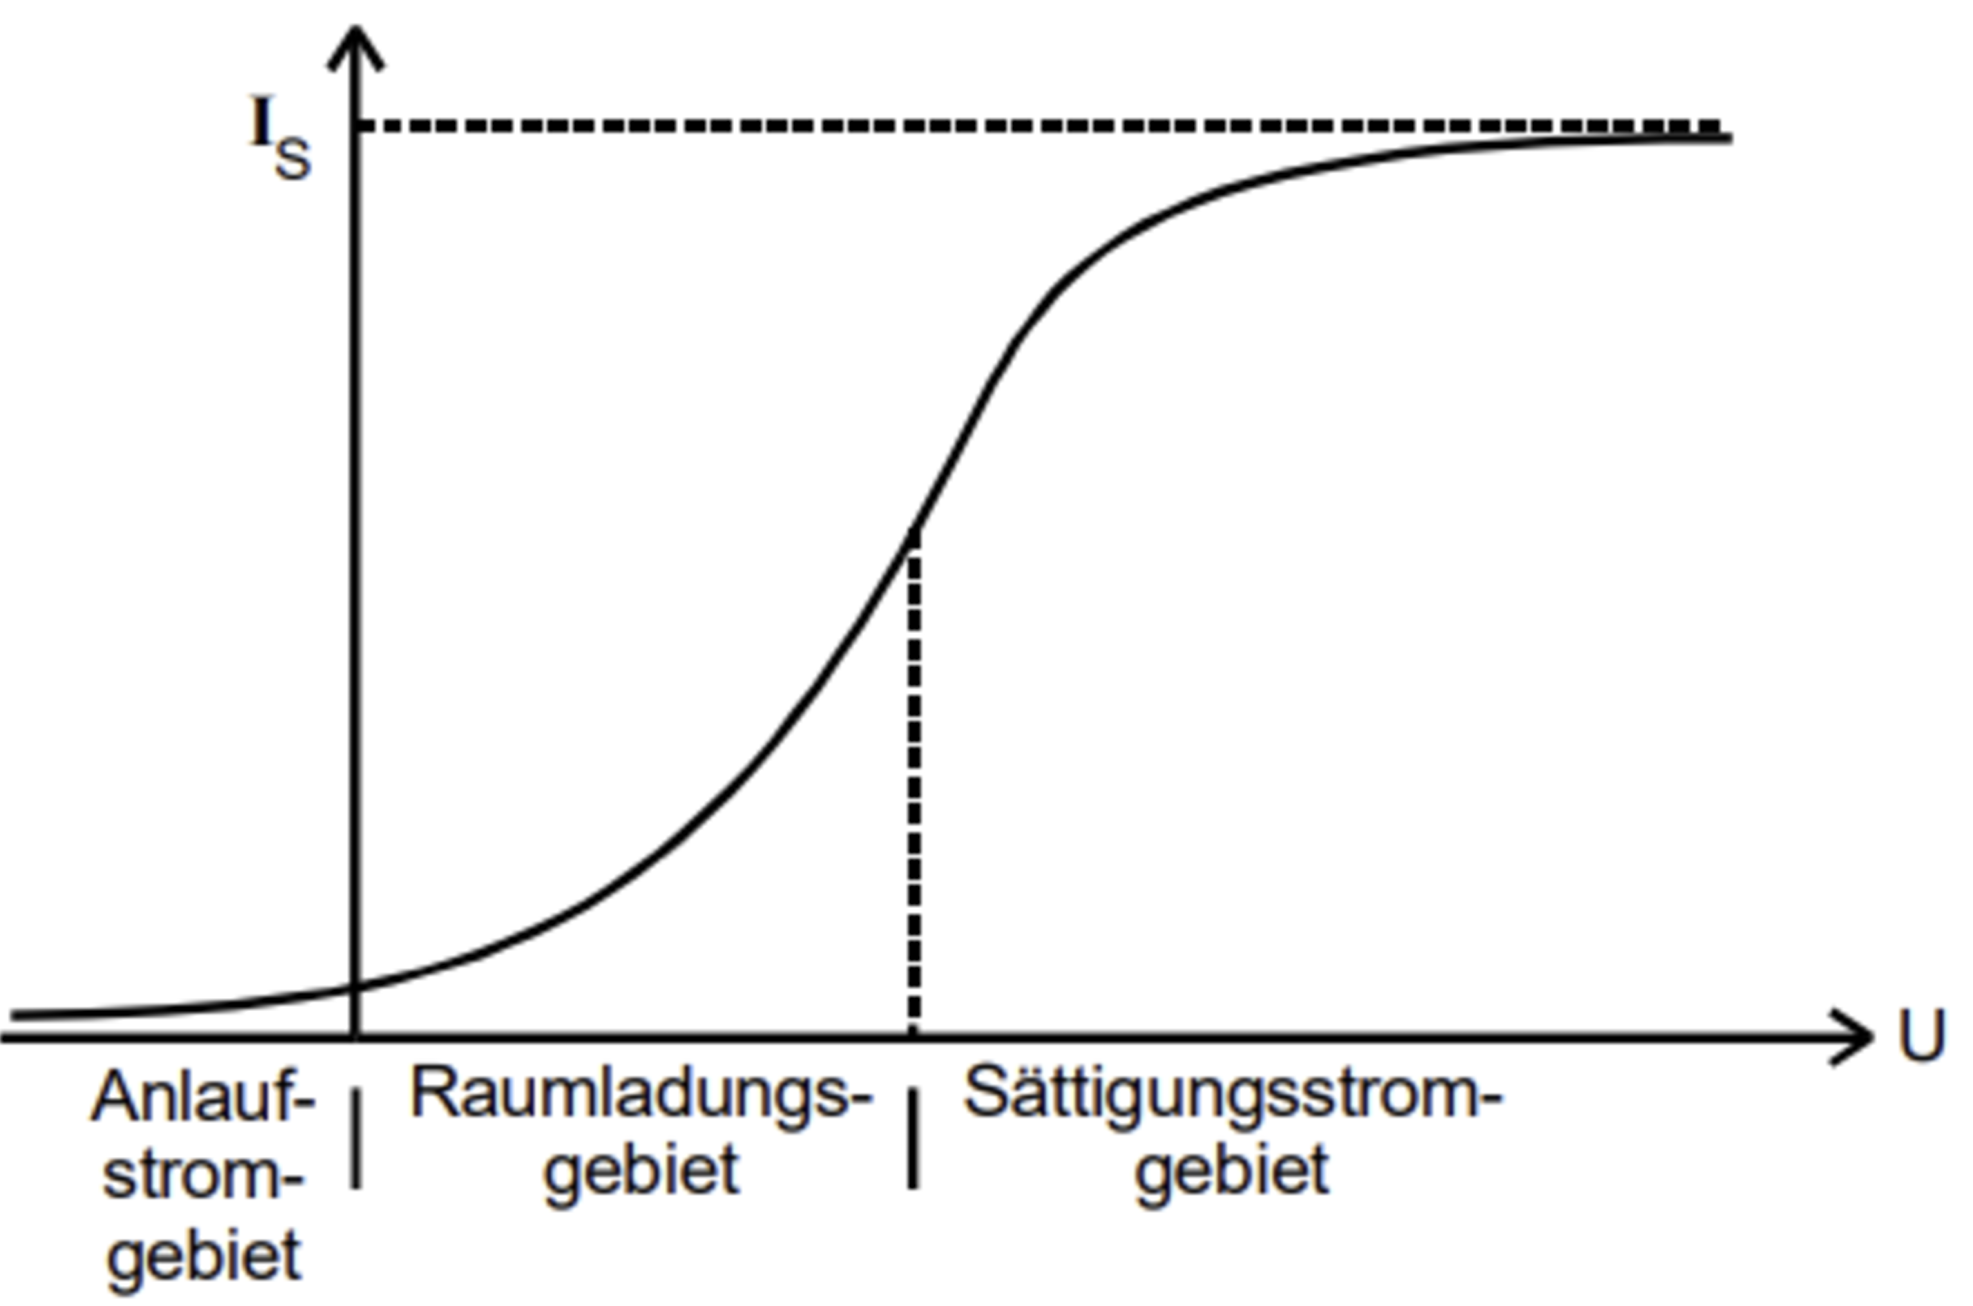
\includegraphics[width=0.9\textwidth]{../build/Kennlinie.pdf}
    \caption{Kennlinie des Geiger-Müller-Zählrohrs.}
\end{figure}




\end{document}
